

The focus of this section is to present the broad overview of research within ADM and its metamodels we have acquired after conducting the systematic review. Moreover, we used information drawn from this overview to answer the research questions. 
\begin{figure*}[t]
\centering
  % Requires \usepackage{graphicx}
  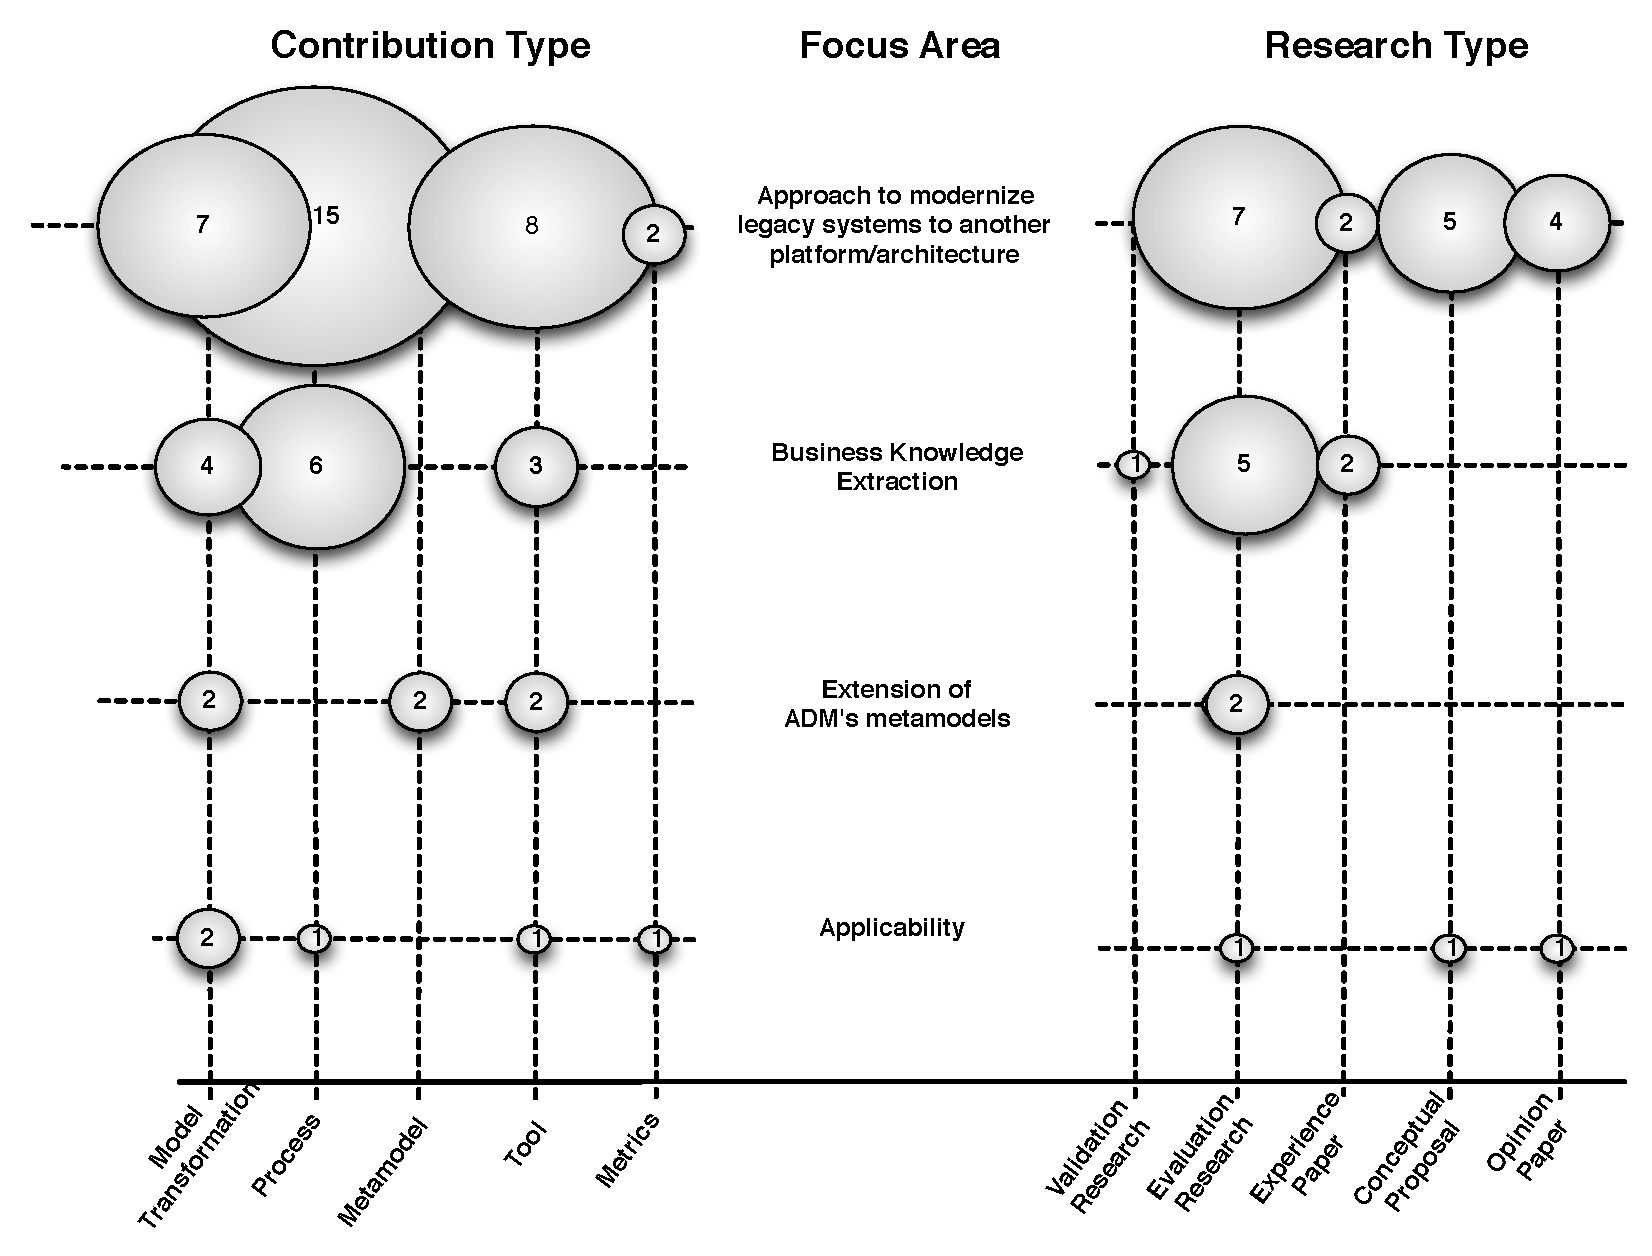
\includegraphics[width=15.5cm, height=6.4cm]{figuras/MapaNOVO3}
\caption{Map of research focus on ADM and its metamodels.}
\label{map}
\end{figure*} 
Aiming to show our results and also the frequencies of all publication related to ADM and its metamodels we plotted a bubble plot, which is depicted in Figure~\ref{map}. Bubble plots are essentially two x-y scatter plots with bubbles in category intersections. The size of each bubble is determined by the number of primary studies that have been classified as belonging to the categories corresponding to the bubble coordinates. This visual summary provides a bird's-eye view that enables one to pinpoint which categories have been emphasized in past research along with gaps and opportunities for future research.

In Figure~\ref{map} the facets we used for organizing the map are the \textbf{contribution type}, \textbf{focus area} and \textbf{research type}. It is worth highlighting that certain primary studies were grouped in more than one category, affecting the frequency count; i.e., the sum of the frequencies shown in each facet can be greater than the total of selected studies presented earlier (30). By observing Figure~\ref{map} can be seen that the majority of research papers are specifically dedicated for providing \textbf{Process} to assist software engineer during the modernization of legacy system to another platform/architecture. Similarly, \textbf{Model transformation} and \textbf{Tool} (to assist ADM's process) are also another field which have been researched. Maybe this came about once the majority of the primary studies found which describe a process to assist the modernization of legacy systems usually propose a set of model transformation and a semi-automatic tool or a fully-automatic one. In contrast, the contribution type with less studies are \textbf{Metamodel} and \textbf{Metrics}. Thus, it is argued that primary studies that describe process to assist the modernization of legacy systems by means of ADM and its metamodels, papers which show a set of rules to be applied during model transformation among the ADM's metamodels (KDM, SMM and ASTM), and papers which devise tools to assist ADM's process are evidence clusters (i.e., where there may be scope for more complete literature reviews to be undertaken), whereas metamodels (i.e., papers that explain how to extend ADM's metamodels) and metrics (i.e., papers which describe how to apply metrics in ADM's metamodel) can be regarded as gaps (i.e., where new or better primary studies are required). In other words, \textbf{Process} to assist software engineer during the modernization of legacy system to another platform/architecture, \textbf{Model transformation} and \textbf{Tool} have been covered by over 43\%, 29\% and 17\%, respectively of the current research (see Figure~\ref{fig:bar}). On the other hand, \textbf{Metamodel} and \textbf{Metrics} have been addressed by a very small number of publications i.e., 3.92\% and 5.88\%, respectively (see Figure~\ref{fig:bar}).   %pieEvaluation

%\begin{figure*}[!h]
% 
%    \subfloat[Frequency of studies in each category.\label{fig:bar}]{
%     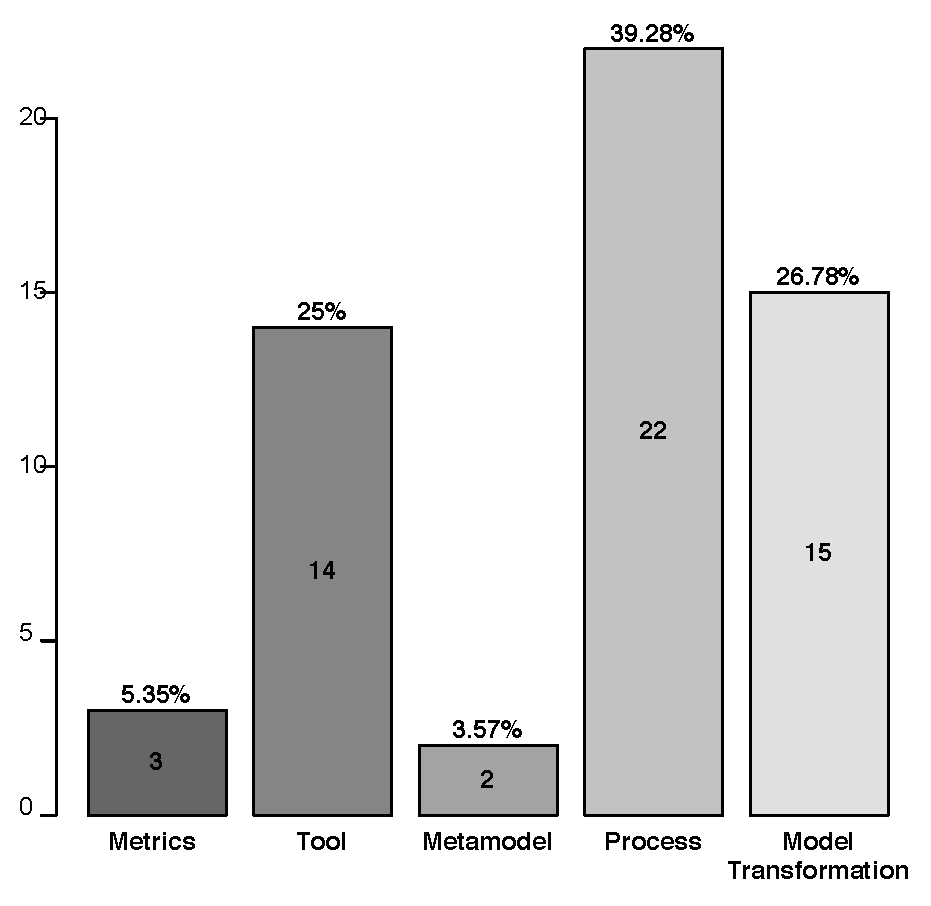
\includegraphics[width=0.2\textwidth]{figuras/NovoBarFormated}
%    }
%    \hfill
%    \subfloat[Frequency of ADM's metamodels used in literature.\label{fig:pie}]{%
%      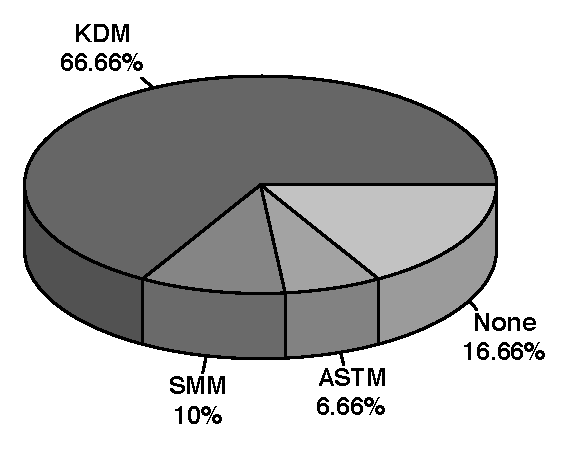
\includegraphics[width=0.2\textwidth]{figuras/pieChartModel}
%    }
%  \hfill
%    \subfloat[Frequency of research type.\label{fig:pieEvaluation}]{%
%      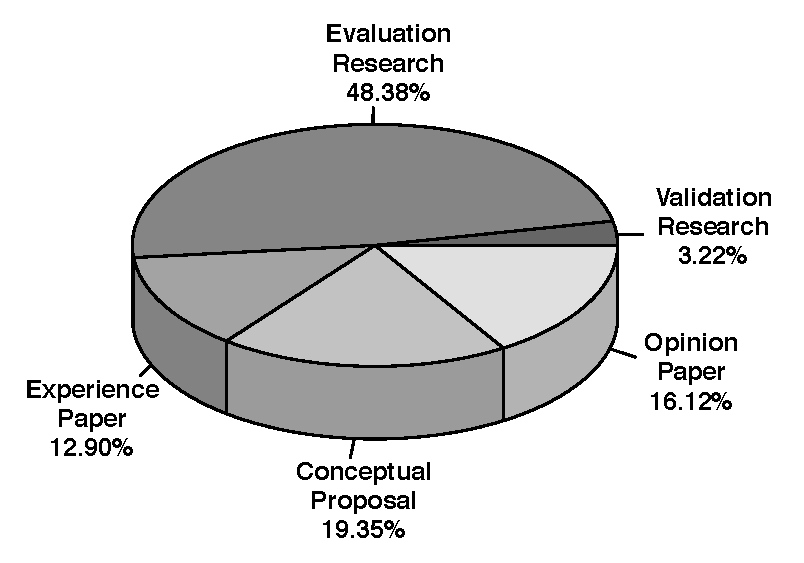
\includegraphics[width=0.25\textwidth]{figuras/pieEvaluation}
%    }
% \hfill
%    \subfloat[ADM standard metamodels used in the literature.\label{fig:pieEvaluation}]{%
%      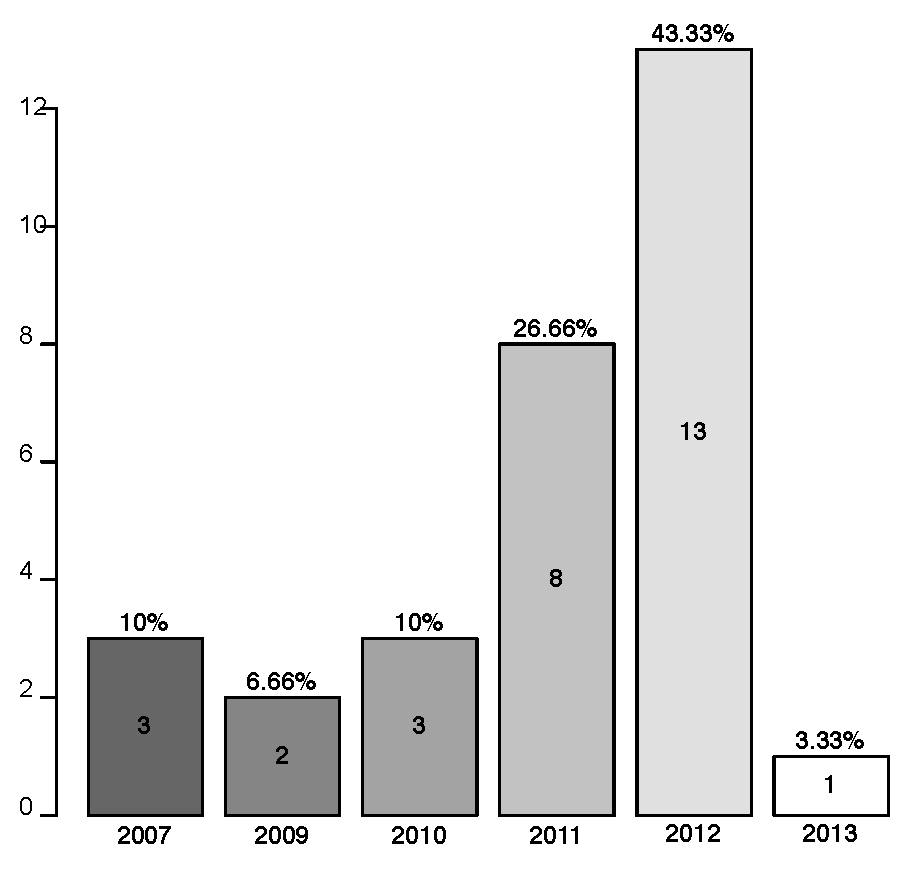
\includegraphics[width=0.2\textwidth]{figuras/DistribuicaoANoArtigos}
%    }
%    \caption{Data gathered.}
%    \label{fig:dummy}
 
% \end{figure*}

%\begin{figure}[!h]
% \centering
  % Requires \usepackage{graphicx}
%  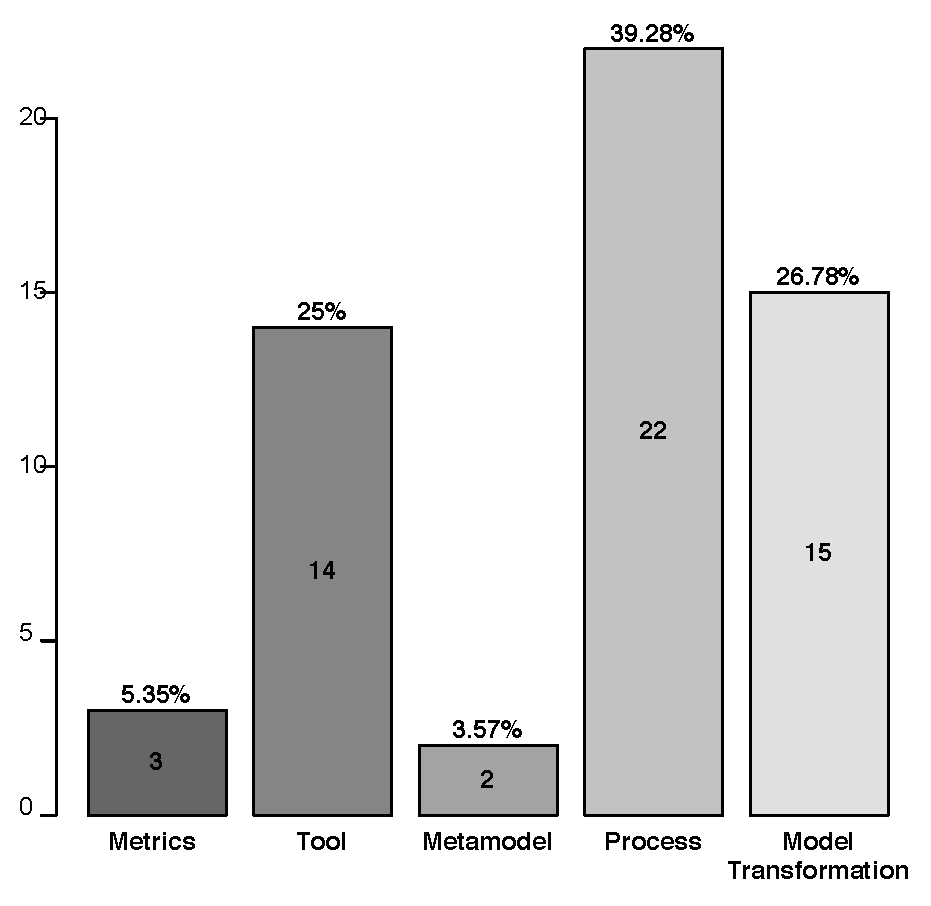
\includegraphics[scale=0.3]{figuras/NovoBarFormated}
% \caption{Frequency of studies in each category.}
% \label{fig:bar}
% \end{figure} %foi esse que eu removi, é o correto...

 As result of this analysis we answered partially the \textbf{RQ$_1$}, i.e., we answered the types of contributions that have been presented so far in liteture related to ADM and its metamodels. Another part of the \textbf{RQ$_1$}, i.e., (a discussion about the focus area regarding the ADM) has been covered in the following Sections~\ref{ssub:approach}-\ref{ssub:applicability}. We have organized each subsection in a way that it briefly describes the studies selected for each topic while highlighting the nature of research.

As for answering the first part of \textbf{RQ$_2$} we analyzed individually all identified primary studies focus on gathering which ADM standard metamodels have more been used in the literature.  In Figure~\ref{fig:pie} is depicted a pie chart wherein we have plotted the collected data. As can be seen in this figure, KDM seems to be the metamodel which has been most used in the literature, covering over 66\%. A small percentage of primary studies have reported on the use of SMM (10\%). While ASTM has been presented by rather small percentage of 6.66\%. Finally, we found out a total of 16.66\% of primary studies that does not show explicitly which metamodel has been used during the process of modernization of a legacy system. In order to answer the second part of \textbf{RQ$_2$} we gathered which are the packages most and least used within the KDM according to the identified studies. In Figure~\ref{fig:piePackage} it is fairly evident that the packages Code and Action are the most used in the literature (65\%). Maybe this came about once these packages are used to represent the source-code of system. Furthermore, the most of the studies found in the literature use somehow the source-code as input to start the modernization process. The third one most used is the Data package (15\%). This package is used to represent relational data, such as database, XML, etc. The packages least used are Event and UI, see Figure~\ref{fig:piePackage}. 

 %\begin{figure}[!h]
 %\centering
  % Requires \usepackage{graphicx}
  % 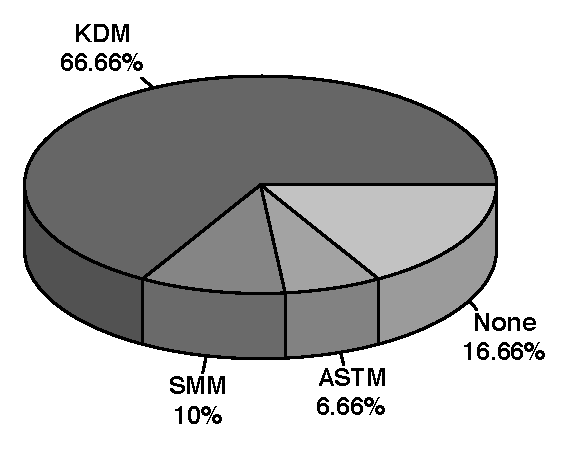
\includegraphics[scale=0.5]{figuras/pieChartModel}
 %\caption{Frequency of ADM's metamodels used in literature.}
 %\label{fig:pie}
%\end{figure} 


\begin{figure}
\def\tabularxcolumn#1{m{#1}}
\begin{tabularx}{\linewidth}{@{}cXX@{}}
%
\begin{tabular}{cc}
\subfloat[\label{fig:pie}]{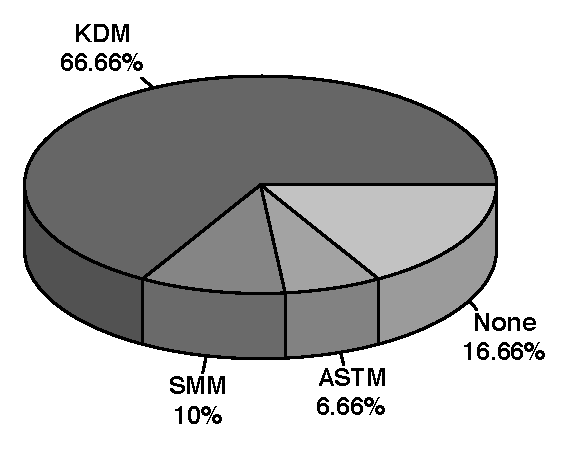
\includegraphics[width=3.9cm]{figuras/pieChartModel}} 
   & \subfloat[\label{fig:piePackage}]{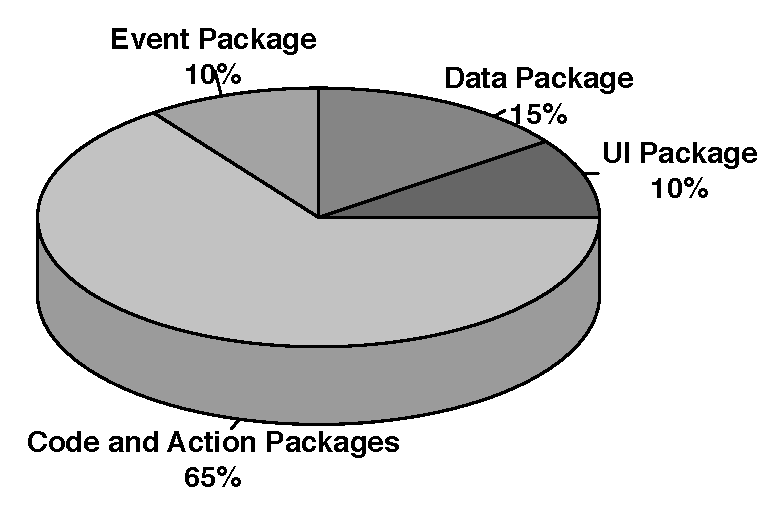
\includegraphics[width=4.5cm]{figuras/PackagesKDMFormatted}}\\
\end{tabular}
\end{tabularx}

\caption{Frequency of ADM's metamodels used in literature and packages most and least used.}\label{foo}
\end{figure}


On the facet \textbf{Research Type}, shows the data we gathered related to the research type employed in the field of ADM (\textbf{RQ$_3$}). As far as the research type is concerned, \textbf{Evaluation Research} are in vast majority, covering 15 primary stydies, see Figure~\ref{map} on the right side. A small number of publications have reported on \textbf{Validation Research} and \textbf{Experience Paper}, i.e., 1 and 4, respectively. While \textbf{Conceptual Proposal}
 and \textbf{Opinion Paper} have been presented collectively by rather of 11 primary studies.
 %Aiming to answer \textbf{RQ$_4$} we collected the name of the conference, name of the journal and the name of the workshop which the primary studies were published, Table~\ref{tab:avenue} covers the second dimension of our results and shows all avenues identified during the conducting of this review. It is fairly evident from observing the Table~\ref{tab:avenue} that the majority of primary studies were published in conference. Therefore, as result the majority of the data related to the systematic review herein were extracted from conference, i.e., among the identified primary studies (30) 23, i.e., 76.66\% studies were published in conference. Even though research has appeared on different conference we can see that in Table~\ref{tab:avenue} that we found out six journals during the review, which represent 20\%, i.e., 6 of the primary studies identified and gathered. The table also reveals that there is only one publication related to ADM and its metamodels that has appeared in a workshop so far.
\begin{figure}
\def\tabularxcolumn#1{m{#1}}
\begin{tabularx}{\linewidth}{@{}cXX@{}}
%
\begin{tabular}{cc}
\subfloat[\label{fig:bar}]{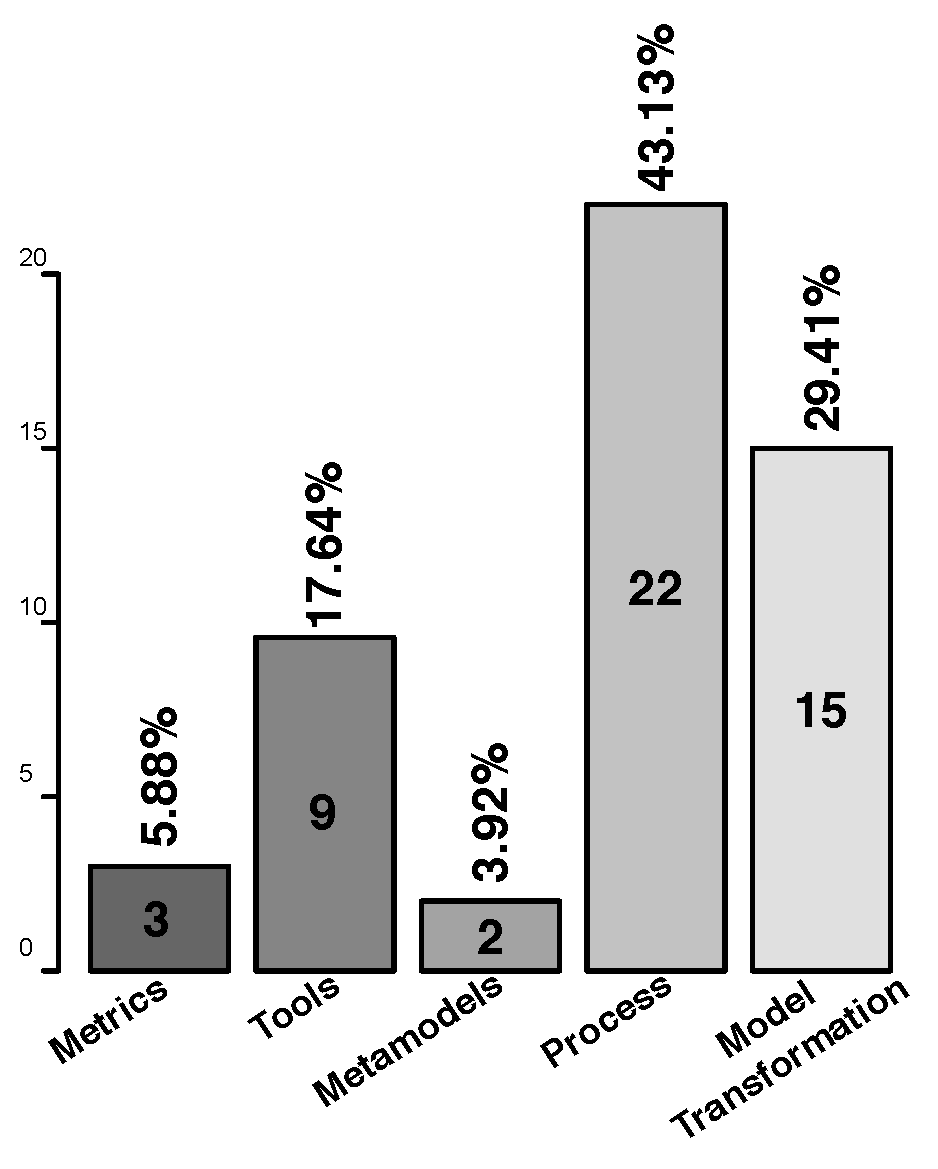
\includegraphics[width=3.9cm]{figuras/TESTEVAI}} 
   & \subfloat[\label{fig:distribuicao_de_artigo_por_ano}]{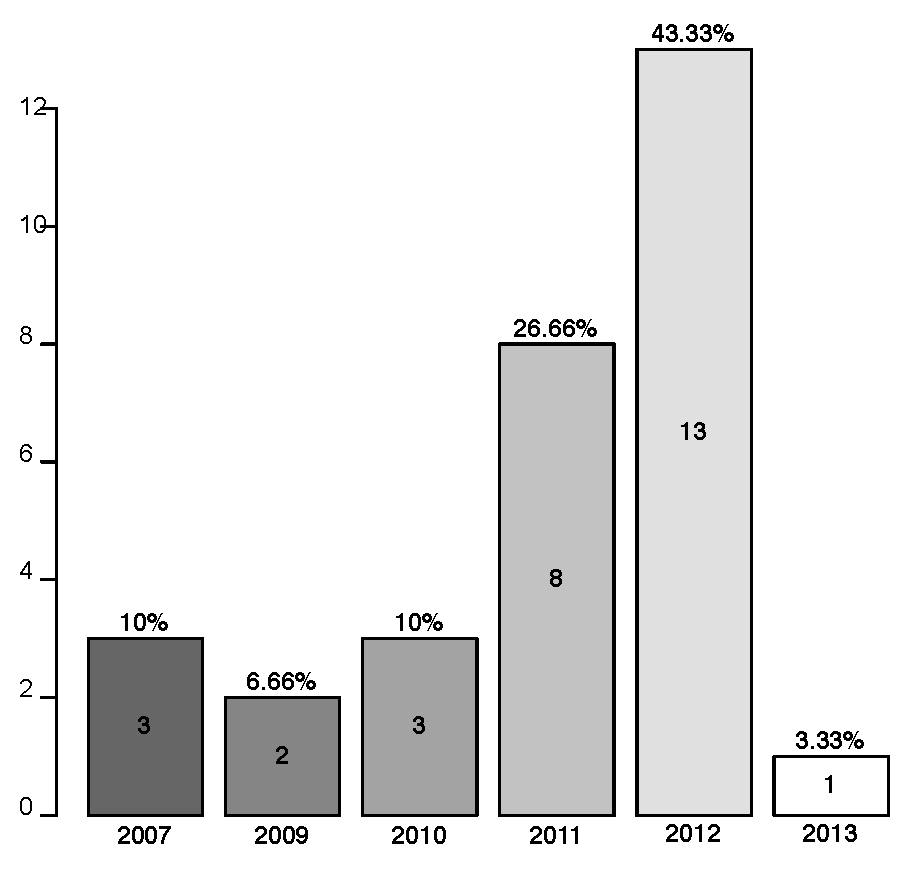
\includegraphics[width=4.2cm]{figuras/DistribuicaoANoArtigos}}\\
\end{tabular}
\end{tabularx}

\caption{Frequency of studies in each category and Distribution of publication by years. }\label{foo}
\end{figure}
 %\begin{figure}[!h]
 %\centering
  % Requires \usepackage{graphicx}
 %  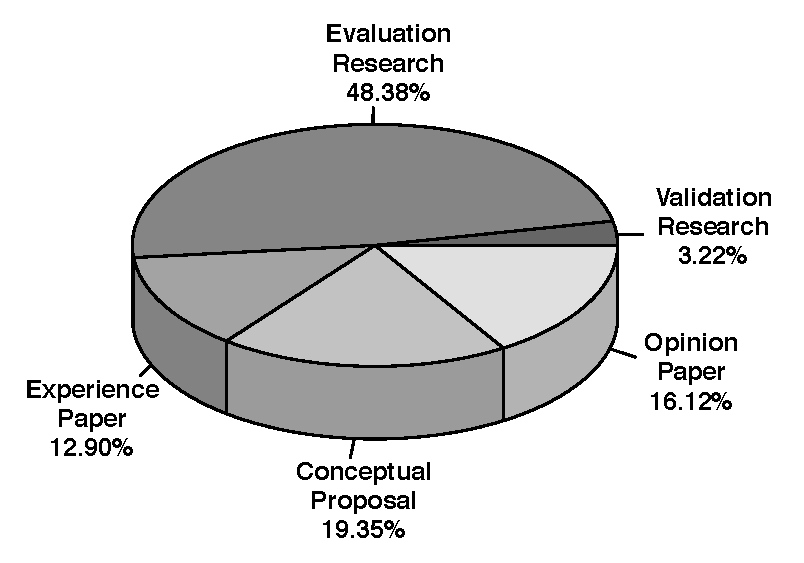
\includegraphics[scale=0.45]{figuras/pieEvaluation}
 %\caption{Frequency of research type.}
% \label{fig:pieEvaluation}
%\end{figure} 
%18 mining techniques for crosscutting concerns, as result we have answered the first part of the RQ$_1$. Based upon this bubble plot, we argue that the answer to second part of the RQ$_1$ is that Fan-In Analysis, Identifier Analysis and Dynamic Analysis are the techniques most used and Program Analysis Based, XScan-Concern-Peers, Data-Flow and Model Driven are the least used. More precisely, among the 62 primary studies included herein, 27 describe Fan-In Analysis, Identifier Analysis or Dynamic Analysis, respectively. In other hands, the techniques with less studies available in literature are Program Analysis Based, XScan-Concern-Peers, Data-Flow and Model Driven. Furthermore, it is argued that Fan-In Analysis, Identifier Analysis and Dynamic Analysis are evidence clusters (i.e., where there may be scope for more complete literature reviews to be undertaken). In contrast, Program Analysis Based, XScan-Concern-Peers, Data-Flow and Model Driven can be deemed as ``evidence desert'' (i.e., wherein better or new research is required). 
Finally, in Figure~\ref{fig:distribuicao_de_artigo_por_ano} shows the distribution by year of the accepted primary studies. As can be seen, the year 2012 had the biggest number of publications related to ADM and its metamodels, i.e., 43.33\%. Among the 30 primary studies included herein 8 were published in 2011, i.e., 26.66\%. In 2007 and in 2010 were published 3 primary studies related to ADM and its metamodelo, representing 20\% of all primary studies. Among the 30 primary studies any of them were published in 2008. In 2009 was identified a percentage of 6.66 of primary studies related to the review herein. Taking into account the search strings was applied in 2013, it may explain the low amount of primary studies published in 2013. 
 %\begin{figure}[!h]
 %\centering
  % Requires \usepackage{graphicx}
  % 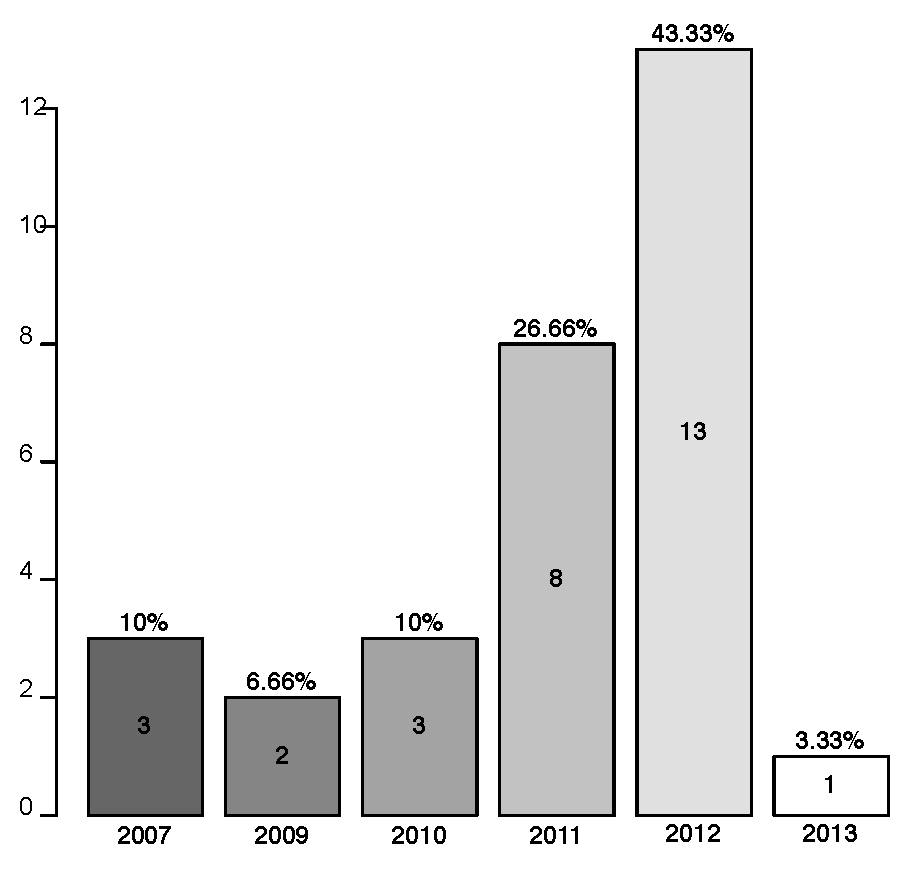
\includegraphics[scale=0.35]{figuras/DistribuicaoANoArtigos}
 %\caption{Distribution of publication by years.}
% \label{fig:distribuicao_de_artigo_por_ano}
%\end{figure} % esse é o correto 
As depicted in second bar of the Figure~\ref{fig:bar}, we identified 9 tools to assist the modernization of legacy systems. In Table~\ref{tab:tools} such tools are named and referenced. By using this table was possible to  answer the fisrt part of the \textbf{RQ$_5$}. As for answering the second part of it, a brief description about the identified tools are presented as follows. 
\begin{table}
\scriptsize
\centering
\caption{The analyzed information of each tool.}
  \begin{tabular}{|l|l|l|}
\hline 
\cellcolor{gray}Name & \cellcolor{gray}Ref & \cellcolor{gray}Website\tabularnewline
\hline 
\hline 
CloudMIG &\cite{SMR:SMR582}  & tinyurl.com/cloudmigxpress\tabularnewline
\hline 
COMO &\cite{5773392}  & No\tabularnewline
\hline 
Gra2MoL &\cite{5440163}  & modelum.es/trac/gra2mol/\tabularnewline
\hline 
MARBLE &\cite{Perez-Castillo:2011:ECS:1982185.1982249,6080834, 6498507,Perez-Castillo:2010:IBP:1875847.1875861,5871783}  & No\tabularnewline
\hline 
MIMOS &~\cite{6498507} & No\tabularnewline
\hline 
MoDisco &~\cite{Bruneliere:2010:MGE:1858996.1859032} & eclipse.org/MoDisco/\tabularnewline
\hline 
PRECISO &~\cite{delCastillo:2009:PRP:1529282.1529753}  & No\tabularnewline
\hline 
R2SOA &~\cite{Guzman:2007:AAR:1339262.1339532} & No\tabularnewline
\hline 
WA2RIA &~\cite{Rodriguez-Echeverria:2011:MLW:2186508.2186536}  & No\tabularnewline
\hline 
\end{tabular}
\label{tab:tools}
\end{table}
\textbf{CloudMIG}. It provides a semi-automatically support for the migration of software systems to PaaS or IaaS-based clouds by using KDM. This tools identifies the possible services by applying a set of rules heuristics., such as: Distribute the five most frequently used services to own virtual machines or The server methods responsible for at least 10\% of overall consumption of the CPU time shall be moved to client side components if they do not need access to the database. After, CloudMIG can generate considerable parts of a resource-efficient target architecture utilizing these rules heuristics~\cite{SMR:SMR582}. 

\textbf{COMO}. It provides an extension to KDM with the concepts of component and interface. By lifting the abstraction level, COMO can produce an adequate view of the entire system, and leverage the boundaries between components to better focus the subsequent modernization effort~\cite{5773392}. This tool neither offer a semi-automatically or automatically way to identify the components, i.e., the engineer has to identify the components.

\textbf{Gra2MoL}. It has been specifically designed to address the problem of extracting models from source code. Gra2MoL is a rule-based transformation language like existing model-to-model transformation languages, but with the fundamental difference that the source element of a rule is a grammar element instead of a source metamodel element~\cite{5440163}. Gra2MoL uses parsers to identify and to extract models from source code.

\textbf{MARBLE}. It is a modernization tool to recover business processes from legacy systems based on KDM. It uses two process mining techniques, static and dynamic analysis of source code to identify business processes. The static one is based on a module that analyze the source code file (Java files in particular) and builds an abstract syntax tree of the source code and then create an instance of KDM. On the other hand, the dynamic one takes the information about the system execution into account to extract meaningful business knowledge.

\textbf{MIMOS}. Similar to MARBLE, MIMOS is a tool to recover business processes from legacy systems based on KDM~\cite{6498507}. This tool uses parser to identify the business processes, then a set of refactoring techniques is applied to KDM.

\textbf{MoDisco}. It aids to offer an open source generic and extensible MDD framework. It aims at providing the required capabilities for creating models and allowing there handling, analysis and computation~\cite{Bruneliere:2010:MGE:1858996.1859032}.

\textbf{PRECISO}. It is a tool for database modernisation through Web Services. Potential services can be simultaneously discovered along with database reverse engineering. A set of patterns are sought in recovered database schema~\cite{delCastillo:2009:PRP:1529282.1529753}.

\textbf{R2SOA}. It is a complete process to reengineer relational databases at a model level to integrate them into SOA contexts as a set of services. Firstly, database schema is reversed and a suitable model is built from the metadata extracted from the database catalog. Based on the structure of the database schema, a first service extraction can be undertaken, a set of model driven pattern matching is used, then CRUD operations are automatically included~\cite{Guzman:2007:AAR:1339262.1339532}.

\textbf{WA2RIA}. It can modernize legacy Web Applications (WA) to Rich Internet Applications (RIAs) by using ADM and KDM. This tool uses MoDisco to get an instance of KDM, then a set of rules are applied to realize the modernization of the WA to RIA~\cite{Rodriguez-Echeverria:2011:MLW:2186508.2186536}.



\subsubsection{Approach to modernize legacy systems to another platform/architecture} % (fold)
\label{ssub:approach}


In this section we briefly describes different studies regarding to propose approaches to modernize legasy systems by means of ADM. Jorge Maratalla et al., propose \textbf{GAFEMO}~\cite{6311013} which aims to modernize a legacy systems to service-oriented approach taking advantage of the features provided by gap-analysis techniques. This approach takes as input a legacy system and then creates KDM representation of it. After, a set of rules are applied in this model to create the services. In~\cite{6080786} the autors present a method that combines ADM with program analysis techniques to support analysis across the components of a component-based system. They builds upon the foundations laid out by OMG's KDM to reverse engineer a homogeneous system-wide dependence model from a software system's heterogeneous source and configuration artifacts, and use this model as the basis for the analysis. In~\cite{Mazon:2007:MDM:1784489.1784497} the authors propose a modernization approach for the modernization of Data warehouses following the concepts of ADM. The approach automatically performs the following tasks: (\textit{i}) obtain a logical representation of data sources (\textit{ii}) mark this logical representation with MD concepts, and (\textit{iii}) derive a conceptual MD model from the marked model. In~\cite{Guzman:2007:AAR:1339262.1339532} is defined an approach which is focused on the analysis of legacy systems to discover and create functionalities to be exposed as services using Web Services. It is based in five steps: (\textit{i}) Database reverse engineering: database schema is reversed and a suitable model is built; (\textit{ii}) First service extraction: based on the structure of the database schema, a first service extraction can be undertaken; (\textit{iii}) PIM generation: is obtained from the PSM representation using a model-to-model transformation, CRUD operations are automatically created; (\textit{iv}) Service discovering: abstract objects are identified in the PIM; (\textit{v}) WSDL (Web Service Description Language) generation: using the PIM, a model-to-model transformation and a WSDL  metamodel are generated to expose the services discovered and created in the PIM and the PSM. In~\cite{5741334, SMR:SMR582} is proposed an approach based on ADM named CloudMIG that aims at supporting SaaS (Software as a Service) providers to semi-automatically migrate legacy software systems to the cloud. It is composed of six major steps: (\textit{i}) Extraction: Includes the extraction of architectural and utilization models of the legacy system, the approach uses KDM; (\textit{ii}) Selection: Select an appropriate CEM- compatible cloud profile candidate; (\textit{iii}) Generation: Produces the target architecture and a mapping model; (\textit{iv}) Adaptation: The adaptation activity enables a reengineer to manually adjust the target architecture; (\textit{v}) Evaluation: Realize static analyses and a runtime simulation of the target architecture; (\textit{vi}) Transformation: The actual transformation of the existing system from the generated target architecture to the aimed cloud environment.

In~\cite{ICEISPerez:CastilloGCP12} is proposed the elicitation of database schemas, a reverse engineering technique that follows the ADM process to recover a minimal relational schema from the queries embedded in the legacy source code. In~\cite{delCastillo:2009:PRP:1529282.1529753} is presented a reengineering process that uses ADM to recover and implement Web Services in automatic manner from relational databases. P\'{e}rez-Castillo et al.,~\cite{5328801} also put forward an approach to modernize legacy systems together with the legacy relational database. This approach recovers the code-to-data linkages and obtains three kinds of models according to the ADM approach: (\textit{i}) The KDM Code Model, which represents the inventory of legacy source code. It has also the points that link the SQL Sentence Models and Database Schema Models. (\textit{ii}) The SQL Sentence Model for modelling a certain SQL query that was embedded in legacy source code. (\textit{iii}) The Database Schema Model, which represents the specific database fragment derived by an SQL Sentence Model. In~\cite{FuentesFernandez2012247} presents the XIRUP modernization methodology, which proposes a highly iterative process, structured into four phases: preliminary evaluation, understanding, building and migration. This modernization process is feature-driven, component-based, focused on the early elicitation of key information, and relies on a ADM.

Mainetti et al.,~\cite{Mainetti:2012:MMT:2364120.2364182} present an approach that allows developers to automatically modernize the client side of legacy systems. In this approach developers can refactor the Graphical User Interface (GUI) of legacy systems during the modernization journey, taking the opportunities offered by novel interaction paradigms, i.e., Rich Internet Application (RIA). Similarly, in~\cite{Rodriguez-Echeverria:2011:MLW:2186508.2186536} the authors present an approach for the definition of a systematic process for Web Applications (WA) to RIA modernization, by applying ADM principles, techniques and tools. The appoach presented by the authors consists on generating a RIA client from the legacy WA presentation and navigation layers and its corresponding service-oriented connection layer with the underlying business logic at server side.

In~\cite{4400179} the authors propose an approach that uses ADM which is focused on the analysis of legacy systems to discover and create functionalities to be exposed as services using Web Services. Boussaidi et al.,~\cite{6385130} propose an approach that makes use of the KDM to reconstruct and document software architectural views of the legacy system. They consider an architectural view to be a way of partitioning a system using a specific set of KDM relevant concepts and relations and they propose clustering algorithms that target specific views mainly a layered view that we call horizontal view and a feature based view that we call vertical view. In~\cite{5440163} ADM is used into practice by building a modernization tool to generate metric reports of legacy Oracle Forms applications to assess migration efforts. The authors devised an extractor that generates KDM models from PL-SQL code (PL/SQL-to-KDM) and a metrics report generator for these KDM models. 

\subsubsection{Business Knowledge Extraction}
\label{ssub:Business_Knowledge_Extraction}

Several papers have contributed to propose approaches to identify Business Knowledge by means of ADM. A brief description of these paper are follows. P\'{e}rez-Castillo et al.,~\cite{Perez-Castillo:2011:ECS:1982185.1982249,6080834, 6498507,Perez-Castillo:2010:IBP:1875847.1875861,5871783} present MARBLE, a modernization tool to recover business processes from legacy systems, as well as two process mining techniques within MARBLE based on static. More specifically, this approach is based on a set of transformation: (\textit{i}) transformation obtains PSM models from each legacy software artifact using a specific metamodel for each artifact, the traditional reverse engineering techniques such as static analysis, dynamic analysis, program slicing and dicing, formal concept analysis, subsystem decomposition, and so on, can be used to extract the needed knowledge; (\textit{ii}) a set of model transformations (e.g. implemented using QVT) to obtain a KDM model built from the PSM models at (\textit{i}); (\textit{iii}) transformation finally obtains the current business process model, this transformation is based on a set of business patterns. In~\cite{PerezCastillo20121370} the authors report the results of a family of case studies that were performed to empirically validate MARBLE using analysis and meta-analysis techniques. The family of case studies demonstrates that the technique is feasible in terms of effectiveness and efficiency. %P\'{e}rez-Castillo et al., also provides in~\cite{} a semi-automatic technique based on dynamic analysis, combined with static analysis to instrument the source code for obtaining event log models. A set of model transformation to transform the event log into another model following the KDM to depict legacy system, concerning its runtime viewpoint, which can be used in any software modernisation project. In~\cite{Perez-Castillo:2010:IBP:1875847.1875861} P\'{e}rez-Castillo et al., explain the KDM2BPMN model transformation within MARBLE, an ADM-based framework to rebuilt business processes embedded in legacy systems in order to facilitate and improve the evolutionary maintenance.

Normantas and Vasilecas ~\cite{lastDAyOFMyLife} present an approach that facilitates software comprehension by enabling traceability of implementation of business rules and business scenarios in the software system, i.e., their approach aim to extract business specific knowledge from the knowledge about the existing software system represented within the KDM. Ropero et al.,~\cite{Fernandez-Ropero:2012:EAB:2367051.2367064} describes a set of rules to transform Mining XML (MXML) metamodel, which is common used to represent the sequence of business activities executed by an enterprise system to KDM. The authors takes an MXML model and obtains an equivalent KDM model at the same abstraction level. The proposed set of rules consist of eight declarative transformation rules. 


\subsubsection{Extension of ADM's metamodels} % (fold)
\label{ssub:extension_of_adm_s_metamodels}

We identified two papers that address how to perform extension of ADM's metamodels. We provided a brief summary of these paper are follows. In~\cite{5773392} the authors propose the COMO (Component-Oriented MOdernization) metamodel an KDM's extension, by borrowing recurring concepts from component-based solutions and software architectures, and to support a proper componentization of the system to assist the modernization of legacy systems. In~\cite{Perez-Castillo:2012:IEL:2231936.2231949} propose an extension to the KDM that aims to represent all the information registered in a MXML model in the KDM model. They claimed that the impact of this extension on well-proven and KDM based tools is not problematic since it is carried out with the own extension mechanism of the KDM standard. Besides this fact, most elements of the event model are present in the core of KDM which is used for many tools.

% subsubsection extension_of_adm_s_metamodels (end)

\subsubsection{Applicability} % (fold)
\label{ssub:applicability}

Similarly, we also identified a small number of papers that address just the applicability of the ADM and its metamodel. Normantas et al.,~\cite{Normantas:2012:OKD:2383276.2383286} where the authors describe all concepts related to the metamodel KDM. The authors claim that the paper enables researchers and practitioners to get a better understanding KDM. P\'{e}rez-Castillo et al.,~\cite{PrezCastillo2011519} present how to use KDM to modernize legacy systems. Also in this paper the authors described each layer of the metamodel KDM, they also presented a set of example of how to use ADM and KDM during the modernization of a legacy systems.

% subsubsection applicability (end)








